\documentclass[11pt,a4paper]{article}
\newcommand{\coursecode}{CIC0101}
\newcommand{\coursename}{Sistemas de Informação}
\newcommand{\lecnumber}{3}
\newcommand{\lectitle}{Entrega 3 - Projeto Integrador}
\newcommand{\lecturer}{Patrícia Araújo de Oliveira}
\newcommand{\semester}{2026 / 2}
\newcommand{\groupnumber}{01}
% ------------- For Encoding & fonts ----------------
\usepackage[T1]{fontenc}
\usepackage[utf8]{inputenc}
\usepackage[brazil]{babel}
\usepackage{lmodern}
\usepackage[scaled=.92]{helvet}   % sans-serif for headings
\usepackage{microtype}

% ---------------- For Layout ----------------
\usepackage[margin=1in, headheight=15pt]{geometry}
\usepackage{setspace}
\setstretch{1.1}
\usepackage{enumitem}
\setlist{itemsep=2pt, topsep=4pt}
\usepackage{booktabs, array, tabularx, graphicx}
\usepackage{caption, subcaption}
\captionsetup{font=small, labelfont={bf,sf}, format=hang}

% ---------------- For Color ----------------
\usepackage[dvipsnames,svgnames]{xcolor}

% ---------------- For Math ----------------
\usepackage{amsmath, amssymb, amsthm, mathtools, bm}

% ---------------- For Boxes ----------------
\usepackage[most]{tcolorbox}

% ------------- For Code & algorithms ----------------
\usepackage{listings}
\usepackage{algorithm}
\usepackage[noend]{algpseudocode}

% -------------- For Figures / plots ----------------
\usepackage{tikz}
\usetikzlibrary{arrows.meta, positioning, shapes.geometric, calc, fit, backgrounds}
\usepackage{pgfplots}
\pgfplotsset{compat=newest}

% ------------- For Headings, headers ----------------
\usepackage{titlesec}
\usepackage{fancyhdr}
\usepackage{lastpage}

% -------- For Hyperlinks (load last) ----------------
\usepackage[colorlinks=true, linkcolor=accent, citecolor=accent3, urlcolor=accent2]{hyperref}

% ---------------- Colors (change the theme here) ----------------
\definecolor{accent}{HTML}{1F5FBF}     % main accent (blue)
\definecolor{accent2}{HTML}{C2410C}    % secondary accent (orange)
\definecolor{accent3}{HTML}{15803D}    % tertiary accent (green)
\definecolor{codebg}{HTML}{F6F8FA}
\definecolor{codegray}{HTML}{6A737D}
\definecolor{codekw}{HTML}{CF222E}
\definecolor{codestr}{HTML}{0A3069}
\definecolor{codefn}{HTML}{8250DF}

% ---------------- Section headings ----------------
\titleformat{\section}{\Large\sffamily\bfseries\color{accent}}{\thesection}{0.7em}{}
\titleformat{\subsection}{\large\sffamily\bfseries\color{black!80}}{\thesubsection}{0.7em}{}
\titleformat{\subsubsection}{\normalsize\sffamily\bfseries\color{black!70}}{\thesubsubsection}{0.7em}{}
\titlespacing*{\section}{0pt}{16pt}{8pt}

% ---------------- Header / footer ----------------
% \pagestyle{fancy}
% \fancyhf{}
% \fancyhead[L]{\sffamily\small\color{gray}\coursecode\ --- \coursename}
% \fancyhead[R]{\sffamily\small\color{gray}Ficha \lecnumber: \lectitle}
% \fancyfoot[C]{\sffamily\small\thepage}
% \renewcommand{\headrulewidth}{0.4pt}
% \renewcommand{\headrule}{\hbox to\headwidth{\color{gray!50}\leaders\hrule height \headrulewidth\hfill}}
\pagestyle{fancy}
\fancyhf{}
\fancyhead[L]{\sffamily\small\color{gray}\coursecode\ --- \coursename}
\fancyhead[R]{\sffamily\small\color{gray}Ficha \lecnumber: \lectitle}
\fancyfoot[L]{\sffamily\small\color{gray}Grupo \groupnumber}
\fancyfoot[C]{\sffamily\small\color{gray}\coursecode\ --- \coursename}
\fancyfoot[R]{\sffamily\small\color{gray}Página \thepage\ de \pageref{LastPage}}
\renewcommand{\headrulewidth}{0.4pt}
\renewcommand{\footrulewidth}{0.4pt}
\renewcommand{\headrule}{\hbox to\headwidth{\color{gray!50}\leaders\hrule height \headrulewidth\hfill}}
\renewcommand{\footrule}{\hbox to\headwidth{\color{gray!50}\leaders\hrule height \footrulewidth\hfill}}

% ---------------- Title block ----------------
\newcommand{\makelecturetitle}{%
  \begin{tcolorbox}[enhanced, colback=accent, colframe=accent, coltext=white,
    sharp corners, boxrule=0pt, left=14pt, right=14pt, top=12pt, bottom=12pt,
    overlay={\fill[white,opacity=0.08] (frame.south east) circle (2.2cm);}]
    {\sffamily\small Universidade de Bras\'ilia\hfill \semester\par}
    {\sffamily\small Departamento de Ci\^encia da Computa\c{c}\~ao\par}
    \vspace{4pt}
    {\sffamily\small\textbf{\coursecode}\ $\cdot$\ \coursename\par}
    \vspace{6pt}
    {\sffamily\bfseries\huge Ficha \lecnumber: \lectitle\par}
    \vspace{6pt}
    {\sffamily\small Professora: \lecturer\hfill Compilado: \today\par}
  \end{tcolorbox}
  \vspace{6pt}
}

% ---------------- Math macros ----------------
\newcommand{\R}{\mathbb{R}}
\newcommand{\N}{\mathbb{N}}
\newcommand{\Z}{\mathbb{Z}}
\newcommand{\E}{\mathbb{E}}
\renewcommand{\Pr}{\mathbb{P}}
% \O already exists in LaTeX (the letter O-slash), so keep it for text mode
% and use \mathcal{O} (Big-O) in math mode.
\let\oslashletter\O
\renewcommand{\O}{\ifmmode\mathcal{O}\else\oslashletter\fi}
\newcommand{\norm}[1]{\left\lVert #1 \right\rVert}
\newcommand{\abs}[1]{\left\lvert #1 \right\rvert}
\newcommand{\inner}[2]{\left\langle #1, #2 \right\rangle}
\DeclareMathOperator*{\argmin}{arg\,min}
\DeclareMathOperator*{\argmax}{arg\,max}

% Nicer QED symbol
\renewcommand{\qedsymbol}{$\blacksquare$}

% Inline code:  \code{merge\_sort(A)}
\newcommand{\code}[1]{\colorbox{codebg}{\texttt{\small #1}}}

\newcommand{\grupointegrantes}[2]{%
  \begin{tcolorbox}[colback=white!92!accent, colbacktitle=accent,
    colframe=accent, coltitle=white, coltext=black,
    title={\sffamily\bfseries #1 --- Integrantes},
    boxrule=0.6pt, arc=1pt, left=14pt, right=14pt, top=6pt, bottom=6pt,
    toptitle=4pt, bottomtitle=4pt]
    \small
    \begin{tabularx}{\linewidth}{@{}>{\raggedright\arraybackslash}X r
                                    >{\raggedright\arraybackslash}X r@{}}
      #2
    \end{tabularx}
  \end{tcolorbox}%
  \vspace{8pt}%
}

% ---------------- Base style for all boxes ----------------
\tcbset{
  thmbase/.style={
    enhanced, breakable, sharp corners, boxrule=0pt, frame hidden,
    left=10pt, right=8pt, top=6pt, bottom=6pt,
    fonttitle=\sffamily\bfseries, before skip=10pt, after skip=10pt
  }
}

% ---------------- Numbered boxes ----------------
% Usage: \begin{theorem}{Title}{label} ... \end{theorem}   ref: Theorem~\ref{thm:label}
\newtcbtheorem[number within=section]{theorem}{Theorem}%
  {thmbase, colback=accent!6, borderline west={3pt}{0pt}{accent}, coltitle=accent}{thm}
\newtcbtheorem[use counter from=theorem]{lemma}{Lemma}%
  {thmbase, colback=accent!6, borderline west={3pt}{0pt}{accent}, coltitle=accent}{lem}
\newtcbtheorem[use counter from=theorem]{definition}{Definition}%
  {thmbase, colback=accent3!7, borderline west={3pt}{0pt}{accent3}, coltitle=accent3}{def}
\newtcbtheorem[use counter from=theorem]{example}{Example}%
  {thmbase, colback=accent2!6, borderline west={3pt}{0pt}{accent2}, coltitle=accent2}{ex}
\newtcbtheorem[number within=section]{exercise}{Exercise}%
  {thmbase, colback=gray!8, borderline west={3pt}{0pt}{gray}, coltitle=black!70}{exc}

% ---------------- Unnumbered boxes ----------------
\newtcolorbox{keyidea}[1][Key Idea]{thmbase, colback=yellow!12,
  borderline west={3pt}{0pt}{yellow!70!orange},
  before upper={\textbf{\sffamily\color{yellow!40!black}#1.}\ }}
\newtcolorbox{notebox}[1][Note]{thmbase, colback=gray!8,
  borderline west={3pt}{0pt}{gray!70},
  before upper={\textbf{\sffamily\color{black!70}#1.}\ }}
\newtcolorbox{warnbox}[1][Warning]{thmbase, colback=red!6,
  borderline west={3pt}{0pt}{red!70!black},
  before upper={\textbf{\sffamily\color{red!70!black}#1.}\ }}
\newtcolorbox{objectives}{thmbase, colback=accent!6,
  borderline west={3pt}{0pt}{accent},
  before upper={\textbf{\sffamily\color{accent}Learning objectives}\par\vspace{2pt}}}

% ---------------- Listings style ----------------
\lstdefinestyle{modern}{
  backgroundcolor=\color{codebg},
  basicstyle=\ttfamily\small,
  commentstyle=\itshape\color{codegray},
  keywordstyle=\bfseries\color{codekw},
  stringstyle=\color{codestr},
  identifierstyle=\color{black},
  numbers=left, numberstyle=\tiny\color{codegray}, numbersep=8pt,
  frame=lines, rulecolor=\color{gray!40},
  framexleftmargin=4pt, xleftmargin=14pt,
  breaklines=true, breakatwhitespace=true,
  postbreak=\mbox{\textcolor{codegray}{$\hookrightarrow$}\space},
  showstringspaces=false, tabsize=4, captionpos=b,
  aboveskip=10pt, belowskip=6pt
}
\lstset{style=modern}

% ---------------- Algorithm style ----------------
\algrenewcommand\algorithmicrequire{\textbf{Input:}}
\algrenewcommand\algorithmicensure{\textbf{Output:}}
\floatname{algorithm}{Algorithm}

\begin{document}
\makelecturetitle
\grupointegrantes{Grupo \groupnumber}{
  \textcolor{accent}{Luan Moura} & \textcolor{accent}{Matrícula não informada} &
  \textcolor{accent}{Leonardo} & \textcolor{accent}{Matrícula não informada} \\
  \textcolor{accent}{Calebe} & \textcolor{accent}{Matrícula não informada} &
  \textcolor{accent}{Maíra} & \textcolor{accent}{Matrícula não informada}
}
\begin{objectives}
Apresentar o modelo conceitual, o Modelo Entidade-Relacionamento (MER), as regras de
negócio, o Diagrama Entidade-Relacionamento (DER) e a consolidação dos dados do
Sistema de Comunicação Escolar, vinculados aos requisitos da Entrega 2.
\end{objectives}
\tableofcontents
\section{Descrição conceitual e regras de negócio}
\begin{notebox}[Questões respondidas]
As respostas abaixo correspondem ao consolidado de respostas do MER elaborado a partir da
Entrega 2, das fichas de MER e DER, dos requisitos funcionais RF01--RF19 e do BPMN do projeto.
\end{notebox}

\subsection{Questão 1 — Pessoa, especializações e nível de acesso}
\textbf{Resposta.} A entidade PESSOA concentra os dados comuns necessários ao sistema:
\texttt{id}, nome, email, telefone, senha\_hash e nivel\_acesso. Ela se especializa de forma exclusiva
em ALUNO, PAIS, PROFESSOR, COORDENADOR ou DIRETOR. Cada especialização é identificada por
\texttt{pessoa\_id}, chave estrangeira que referencia PESSOA.

ALUNO possui matricula; PAIS possui grau\_parentesco; PROFESSOR possui registro\_funcional;
COORDENADOR possui setor; DIRETOR não exige atributos próprios além dos dados herdados.
O nivel\_acesso define permissões, segmentação dos avisos e visualização do feed.

\subsection{Questão 2 — Turma}
\textbf{Resposta.} TURMA representa uma divisão acadêmica organizada pela escola. Seus atributos são
\texttt{id}, \texttt{professor\_orientador\_id}, nome, ano, turno, inicio\_vigencia e fim\_vigencia.
O atributo professor\_orientador\_id referencia PROFESSOR. Uma turma possui um professor orientador
e pode oferecer uma ou mais disciplinas.

\subsection{Questão 3 — Disciplina}
\textbf{Resposta.} DISCIPLINA corresponde aos componentes curriculares comunicados pela escola.
Possui \texttt{id}, nome e codigo. Uma disciplina pode estar associada a uma ou mais turmas,
dependendo da organização acadêmica do período.

\subsection{Questão 4 — Oferta acadêmica e horários}
\textbf{Resposta.} TURMA, DISCIPLINA e PROFESSOR se relacionam pela entidade associativa
TURMA\_DISCIPLINA\_PROFESSOR\_HORARIO. Cada registro associa turma, disciplina e professor.
Essa entidade se relaciona com HORARIO, que possui \texttt{id}, dia\_semana, hora\_inicio e
hora\_fim. O dia da semana é limitado a SEGUNDA, TERCA, QUARTA, QUINTA ou SEXTA.
Uma turma pode possuir várias ofertas, uma disciplina pode ser ministrada em várias turmas,
um professor pode ministrar várias ofertas e cada oferta pode possuir um ou mais horários.

\subsection{Questão 5 — Matrícula na turma}
\textbf{Resposta.} ALUNO e TURMA se relacionam pela entidade associativa ALUNO\_TURMA.
Cada registro contém \texttt{aluno\_id}, \texttt{turma\_id}, data\_matricula e status\_matricula.
As duas chaves juntas identificam de forma única o vínculo entre estudante e turma.
Um aluno pode estar vinculado a várias turmas ao longo da trajetória escolar, e uma turma
pode conter vários alunos.

\subsection{Questão 6 — Categoria de aviso}
\textbf{Resposta.} CATEGORIA\_AVISO agrupa os avisos conforme sua finalidade institucional.
Possui \texttt{id}, nome e exige\_moderacao. Uma categoria pode classificar vários avisos, mas
cada aviso pertence a uma única categoria. exige\_moderacao determina se o fluxo de aprovação
institucional deve ser iniciado antes da publicação.

\subsection{Questão 7 — Aviso}
\textbf{Resposta.} AVISO representa a comunicação criada e distribuída pelo sistema. Seus atributos
são \texttt{id}, autor\_id, categoria\_id, titulo, descricao, formato, url, nivel\_urgencia,
data\_criacao, data\_publicacao e status. Cada aviso é criado por uma pessoa e vinculado a uma
categoria. O status registra elaboração, aguardo de avaliação, aprovação, publicação ou rejeição.

\subsection{Questão 8 — Solicitação de autorização}
\textbf{Resposta.} SOLICITACAO\_AUTORIZACAO registra o fluxo de aprovação dos avisos sujeitos à
moderação. Possui \texttt{id}, aviso\_id, avaliador\_id, data\_solicitacao, data\_avaliacao,
decisao e feedback. Cada solicitação pertence a um único aviso e a um único avaliador.
Um aviso pode gerar várias solicitações, preservando correções, novas avaliações e decisões.

\subsection{Questão 9 — Envio}
\textbf{Resposta.} ENVIO representa a operacionalização da distribuição de um aviso liberado.
Possui \texttt{id}, aviso\_id, data\_envio, canal e tipo\_segmentacao. Um aviso pode gerar
um ou mais envios. O canal indica o meio utilizado, e tipo\_segmentacao indica se o público foi
definido por turma, grupo, função ou seleção específica.

\subsection{Questão 10 — Destinatários da segmentação}
\textbf{Resposta.} ENVIO\_DESTINATARIO representa o relacionamento n:m entre ENVIO e PESSOA.
Cada registro usa envio\_id e pessoa\_id como chave composta. Um envio pode ser direcionado
a várias pessoas, e uma pessoa pode receber vários envios.

\subsection{Questão 11 — Controle de recebimento}
\textbf{Resposta.} CONTROLE\_RECEBIMENTO registra a interação dos destinatários com cada envio.
Possui \texttt{id}, envio\_destinatario\_envio\_id, envio\_destinatario\_pessoa\_id,
data\_visualizacao e data\_recebimento. Cada registro está associado a um único par envio-destinatário
e mantém o histórico de entrega e visualização. O perfil é obtido por PESSOA.nivel\_acesso.

\section{Entidades, atributos e identificadores do MER}
\begin{table}[!ht]\centering\scriptsize\renewcommand{\arraystretch}{1.45}
\begin{tabularx}{\linewidth}{|>{\raggedright\arraybackslash}p{3.1cm}|>{\raggedright\arraybackslash}X|>{\raggedright\arraybackslash}p{2.7cm}|>{\raggedright\arraybackslash}p{2.1cm}|}
\hline
\textbf{Entidade} & \textbf{Atributos necessários} & \textbf{Identificador} & \textbf{RF} \\
\hline
PESSOA & usuario, email, nome, cpf, telefone, senha\_hash, nivel\_acesso\_id & id & 01,05,11,19 \\
\hline ALUNO & matricula, serie, pessoa\_id & pessoa\_id & 03,19 \\
\hline RESPONSAVEL & telefone\_emergencia, pessoa\_id & pessoa\_id & 01,04 \\
\hline FUNCIONARIO & registro\_funcional, tipo, pessoa\_id & pessoa\_id & 05,06,11,15 \\
\hline NIVEL\_ACESSO & descricao, permissões do perfil & id & 06,10 \\
\hline TURMA & nome, ano, sala, inicio\_vigencia, fim\_vigencia & id & 03 \\
\hline DISCIPLINA & nome, codigo & id & 03 \\
\hline ALUNO\_TURMA & data\_matricula, status\_matricula & aluno\_id + turma\_id & 03 \\
\hline OFERTA\_ACADEMICA & turma, disciplina, professor, dias, turnos, horários & id & 03 \\
\hline NOTA & valor, nome\_avaliacao, data\_lancamento & id & 03,19 \\
\hline FREQUENCIA & data\_aula, status\_presenca & id & 03,19 \\
\hline AVISO & autor, titulo, descricao, formato, url, urgência, datas, status & id & 02,03,15,16,17 \\
\hline AVISO\_SEGMENTACAO & aviso, tipo\_alvo, alvo\_id & id & 03 \\
\hline MENSAGEM & remetente, destinatario, titulo, descricao, formato, tipo, status & id & 01,05,11,12,13 \\
\hline RESPOSTA\_MENSAGEM & mensagem, titulo, descricao, data\_criacao & id & 14,18 \\
\hline AUTORIZACAO\_AVISO & aviso, avaliador, datas, status, feedback & id & 06--10,15 \\
\hline ENVIO & aviso, data\_envio, canal, tipo\_segmentacao & id & 04,16 \\
\hline ENVIO\_DESTINATARIO & envio\_id, pessoa\_id & envio\_id + pessoa\_id & 03,19 \\
\hline VISUALIZACAO & aviso, pessoa, data\_hora\_visualizacao & aviso\_id + pessoa\_id & 11,19 \\
\hline REACAO\_AVISO & aviso, pessoa, tipo & aviso\_id + pessoa\_id & 19 \\
\hline COMENTARIO & aviso, pessoa, texto, data\_criacao & id & 19 \\
\hline\end{tabularx}
\end{table}

\section{Relacionamentos e regras de negócio}
\begin{table}[!ht]\centering\scriptsize\renewcommand{\arraystretch}{1.38}
\begin{tabularx}{\linewidth}{|>{\raggedright\arraybackslash}p{2.9cm}|>{\centering\arraybackslash}p{1.4cm}|>{\raggedright\arraybackslash}p{2.8cm}|>{\raggedright\arraybackslash}X|}
\hline
\textbf{Entidade A} & \textbf{Verbo} & \textbf{Entidade B} & \textbf{Regra ou dúvida a validar} \\
\hline
NIVEL\_ACESSO & define & PESSOA & Permissões de criar mensagens, distribuir avisos e visualizar o feed. \\
\hline RESPONSAVEL & possui & PARENTESCO & Grau de parentesco e número máximo de responsáveis por aluno. \\
\hline ALUNO & possui & PARENTESCO & Como validar vínculo de responsabilidade legal. \\
\hline FUNCIONARIO & orienta & TURMA & Um professor pode orientar mais de uma turma. \\
\hline ALUNO & matricula-se em & ALUNO\_TURMA & Status: matriculado, transferido, concluído ou desmatriculado. \\
\hline TURMA & engloba & ALUNO\_TURMA & Capacidade máxima da turma. \\
\hline TURMA & possui & OFERTA\_ACADEMICA & Estrutura da grade e dos horários do período letivo. \\
\hline DISCIPLINA & compõe & OFERTA\_ACADEMICA & Uma disciplina pode ser oferecida várias vezes. \\
\hline FUNCIONARIO & ministra & OFERTA\_ACADEMICA & Coexistência de mais de um professor na mesma oferta. \\
\hline OFERTA\_ACADEMICA & registra & NOTA & Critérios, etapas e pesos das avaliações. \\
\hline ALUNO & recebe & NOTA & Forma de consulta ao boletim pelo aluno e responsável. \\
\hline OFERTA\_ACADEMICA & controla & FREQUENCIA & Frequência diária ou consolidada por período. \\
\hline ALUNO & acumula & FREQUENCIA & Cálculo da presença mínima e faltas justificadas. \\
\hline FUNCIONARIO & cria & AVISO & Categorias com autonomia e categorias sujeitas a moderação. \\
\hline AVISO & segmenta & AVISO\_SEGMENTACAO & Direcionamento por turma, série, perfil ou toda a escola. \\
\hline AVISO & pode requerer & AUTORIZACAO\_AVISO & Regra baseada em categoria ou nível de acesso. \\
\hline FUNCIONARIO & avalia & AUTORIZACAO\_AVISO & Possibilidade de solicitar ajustes antes da aprovação. \\
\hline RESPONSAVEL & envia & MENSAGEM & Direcionamento da demanda ao setor competente. \\
\hline FUNCIONARIO & recebe & MENSAGEM & Notificação em tempo real no sistema ou externamente. \\
\hline MENSAGEM & possui & RESPOSTA\_MENSAGEM & Fluxo linear ou diálogo encadeado. \\
\hline AVISO & gera & ENVIO & Canais externos acionados automaticamente na publicação. \\
\hline ENVIO & direciona & ENVIO\_DESTINATARIO & Como o público é resolvido e atualizado. \\
\hline PESSOA & registra & VISUALIZACAO & Carimbo de data/hora e confirmação de ciência. \\
\hline AVISO & recebe & REACAO\_AVISO & Tipos de reação permitidos e alteração posterior. \\
\hline AVISO & contém & COMENTARIO & Existência de moderação e permissão de exclusão. \\
\hline\end{tabularx}
\end{table}

\section{Cardinalidades consolidadas do DER}
\begin{table}[!ht]\centering\scriptsize\renewcommand{\arraystretch}{1.42}
\begin{tabularx}{\linewidth}{|>{\raggedright\arraybackslash}p{4.0cm}|>{\centering\arraybackslash}p{1.45cm}|>{\centering\arraybackslash}p{1.45cm}|>{\raggedright\arraybackslash}X|}
\hline
\textbf{Relacionamento} & \textbf{A $\rightarrow$ B} & \textbf{B $\rightarrow$ A} & \textbf{Justificativa} \\
\hline
NIVEL\_ACESSO --- define --- PESSOA & 1:N & N:1 & Um nível pode ser atribuído a várias pessoas. \\
\hline PESSOA --- especializa --- ALUNO/RESPONSAVEL/FUNCIONARIO & 1:1 & 1:1 & Especialização exclusiva por perfil. \\
\hline ALUNO --- participa --- ALUNO\_TURMA --- pertence --- TURMA & 1:N & N:1 & Histórico de matrículas em turmas. \\
\hline TURMA --- possui --- OFERTA\_ACADEMICA & 1:N & N:1 & Uma turma possui várias ofertas. \\
\hline DISCIPLINA --- compõe --- OFERTA\_ACADEMICA & 1:N & N:1 & Uma disciplina pode aparecer em várias ofertas. \\
\hline FUNCIONARIO --- ministra --- OFERTA\_ACADEMICA & 1:N & N:1 & Um professor pode ministrar várias ofertas. \\
\hline OFERTA\_ACADEMICA --- registra --- NOTA & 1:N & N:1 & Uma oferta contém várias avaliações. \\
\hline OFERTA\_ACADEMICA --- controla --- FREQUENCIA & 1:N & N:1 & Várias frequências são registradas por oferta. \\
\hline FUNCIONARIO --- cria --- AVISO & 1:N & N:1 & Uma pessoa cria vários avisos. \\
\hline CATEGORIA\_AVISO --- classifica --- AVISO & 1:N & N:1 & Cada aviso possui uma categoria. \\
\hline AVISO --- possui --- AUTORIZACAO\_AVISO & 1:N & N:1 & Correções podem gerar novas solicitações. \\
\hline AVISO --- gera --- ENVIO & 1:N & N:1 & Um aviso pode ser enviado em diferentes canais ou momentos. \\
\hline ENVIO --- direciona --- ENVIO\_DESTINATARIO --- Pessoa & N:M & M:N & Segmentação de vários destinatários por envio. \\
\hline ENVIO\_DESTINATARIO --- possui --- CONTROLE\_RECEBIMENTO & 1:1 & 1:1 & Um par envio-destinatário possui um controle consolidado. \\
\hline AVISO --- recebe --- VISUALIZACAO & 1:N & N:1 & Várias pessoas podem visualizar um aviso. \\
\hline PESSOA --- envia --- MENSAGEM & 1:N & N:1 & Uma pessoa pode enviar várias mensagens. \\
\hline PESSOA --- recebe --- MENSAGEM & 1:N & N:1 & Uma pessoa pode receber várias mensagens. \\
\hline MENSAGEM --- possui --- RESPOSTA\_MENSAGEM & 1:N & N:1 & Uma mensagem pode ter resposta oficial ou histórico de respostas. \\
\hline AVISO --- segmenta --- AVISO\_SEGMENTACAO & 1:N & N:1 & Um aviso pode atingir vários públicos. \\
\hline\end{tabularx}
\end{table}

\section{DER conceitual e modelo lógico}
\begin{figure}[!ht]
\centering
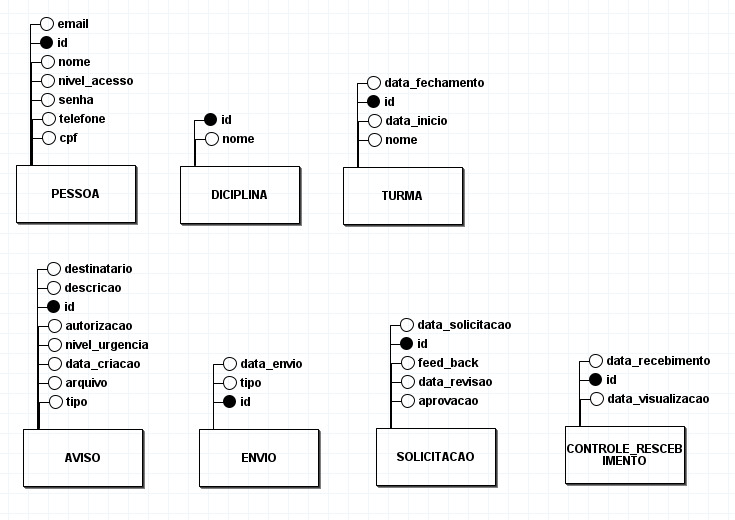
\includegraphics[width=\linewidth,height=0.62\textheight,keepaspectratio]{../../src/uml/diagrama/der.jpeg}
\caption{DER consolidado do Sistema de Comunicação Escolar.}
\end{figure}

\begin{figure}[!ht]
\centering
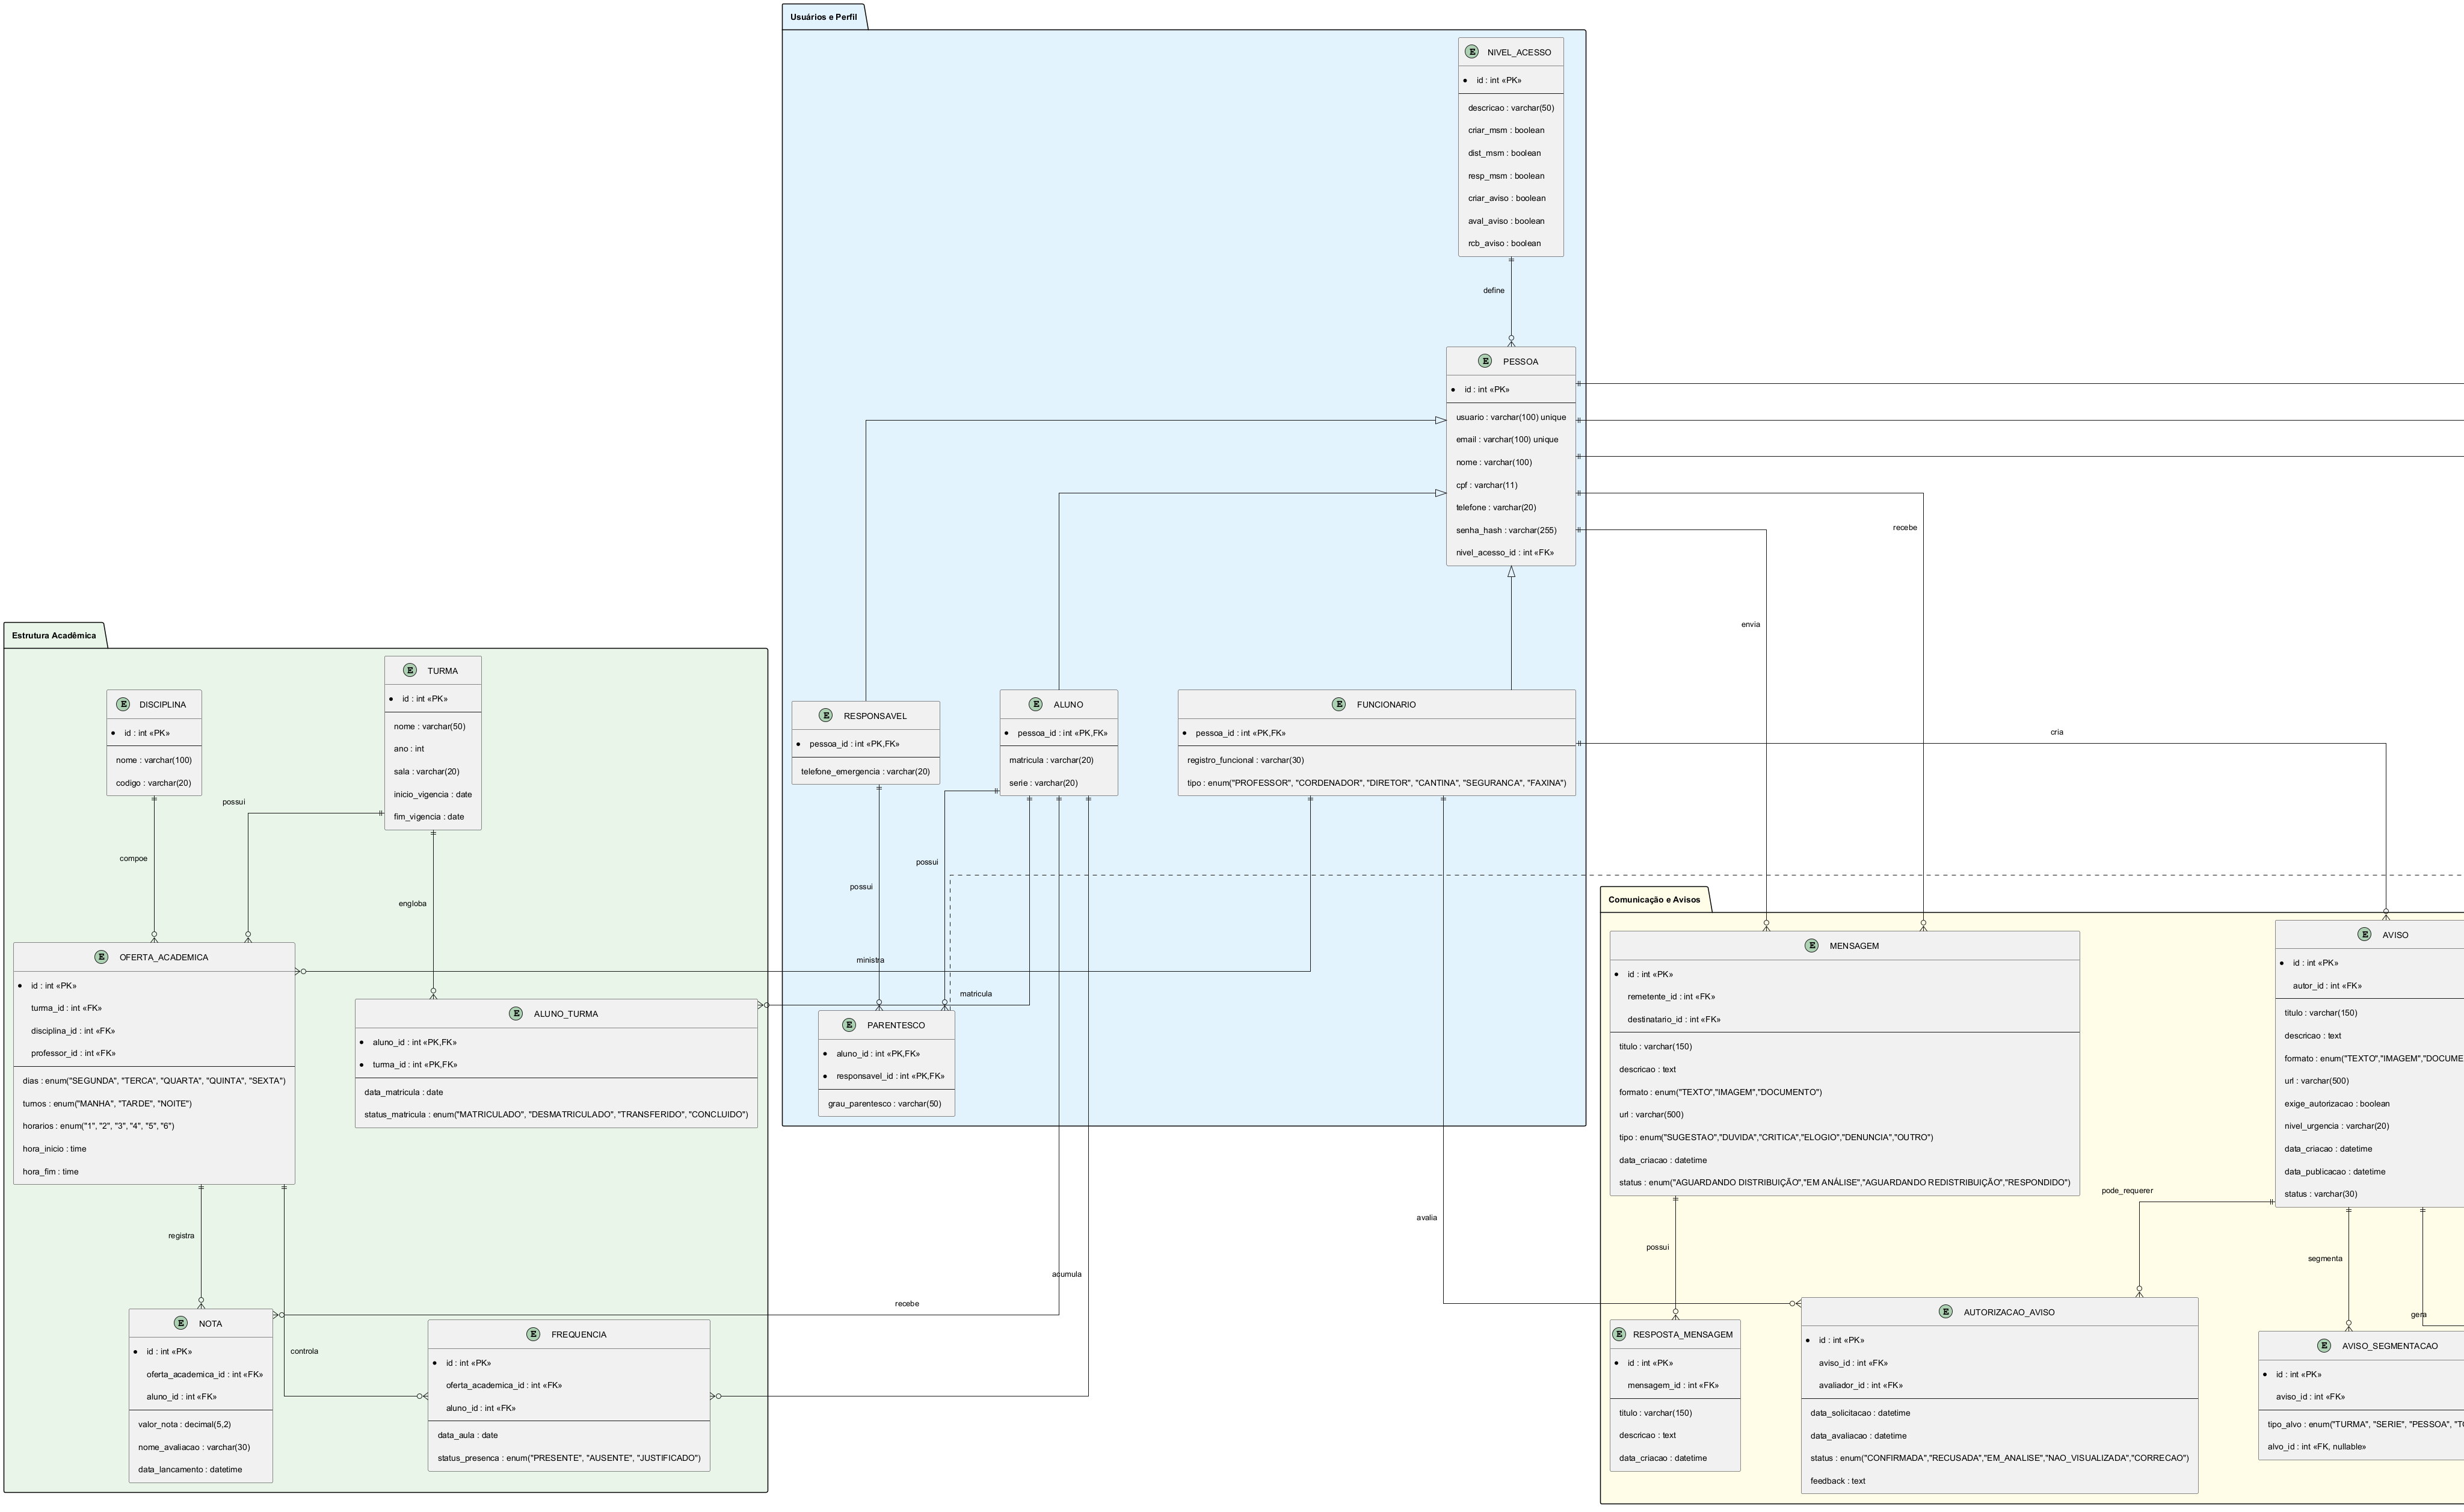
\includegraphics[width=\linewidth,height=0.62\textheight,keepaspectratio]{../../src/uml/logico/mr.png}
\caption{Modelo Relacional derivado do MER conceitual.}
\end{figure}

\begin{keyidea}[Chaves das entidades associativas]
ALUNO\_TURMA usa aluno\_id e turma\_id; ENVIO\_DESTINATARIO usa envio\_id e pessoa\_id;
CONTROLE\_RECEBIMENTO mantém referência ao par envio-destinatário. Tais entidades associativas
representam corretamente os relacionamentos muitos para muitos.
\end{keyidea}

\section{Verificação de rastreabilidade e coerência}
\begin{table}[!ht]\centering\small\renewcommand{\arraystretch}{1.5}
\begin{tabularx}{\linewidth}{|>{\raggedright\arraybackslash}p{4cm}|>{\raggedright\arraybackslash}X|}
\hline
\textbf{Ponto de verificação} & \textbf{Resposta do grupo} \\
\hline
Os requisitos foram considerados? & Todos os RF01--RF19 possuem dados ou relacionamentos associados no MER, no DER ou nas entidades associativas. \\
\hline
Os identificadores estão definidos? & Cada entidade possui chave própria; os relacionamentos muitos para muitos são representados por chaves compostas. \\
\hline
As regras de negócio estão registradas? & Moderação, segmentação, recebimento, parentesco, matrícula, grade acadêmica e mensagens possuem regras e dúvidas de validação. \\
\hline
Existem entidades sem uso rastreável? & REACAO\_AVISO e COMENTARIO estão ligados ao RF19; NOTA e FREQUENCIA ampliam o acompanhamento acadêmico. \\
\hline
O modelo mantém o problema de origem? & O MER concentra comunicação centralizada, moderação, segmentação, entrega, recebimento, atendimento e acompanhamento escolar. \\
\hline
Quais pontos precisam ser validados? & Categorias sujeitas à moderação; vínculo entre responsáveis e alunos; canais externos; confirmação de leitura; comentários; horários e avaliações acadêmicas. \\
\hline
\end{tabularx}
\end{table}

\begin{objectives}
\textbf{Conclusão.} O modelo conceitual derivado da Entrega 2 e das fichas de MER/DER representa
as entidades necessárias ao funcionamento do sistema. Os diagramas foram preservados e as regras
de negócio foram organizadas como respostas às atividades solicitadas pela professora.
Pontos dependentes da validação institucional permanecem explicitamente registrados.
\end{objectives}

\end{document}
